\chapter{Design and Prototyping}\label{ch:DesProt}
\vspace{-2.5em}
% \newthought{Synopsis}\synopsisChProcessing
\newthought{Synopsis}\synopsisDesign
\mynewline
\section{Conceptualisation and Initial Design}
The essence of a design process is inherently iterative and exploratory. It's a cyclical journey of conception, experimentation, evaluation, and refinement. This iterative cycle is fundamental to translating abstract ideas into tangible solutions that meet specific functional and operational goals.
%Within this framework, the development of a mock \gls{TV} for a heart simulator exemplifies the complex interplay of innovation, precision, and adaptability.

At the heart of the design process lies the concept of trial and error—a methodical yet flexible approach that takes the discovery of unexpected challenges and leverages them as opportunities for learning. Initial ideas are transformed into preliminary models, serving as the first step in a series of continuous interactions between designing, testing, and iterating.
%This process is characterized by the application of various modeling approaches, each iteration informed by the insights gained from previous attempts and the evolving understanding of the project's objectives.

The dynamic nature of this process sets a strong base to pivot strategies, incorporate new technologies, and adapt to findings in real-time. The design changes throughout this project were not merely reactions to setbacks but were driven by a pursuit of optimization—whether in response to material limitations, fabrication challenges, or new anatomical insights.
% Reworking based on these design changes is critical, allowing the prototypes to improve incrementally, each iteration bringing them closer to the optimal balance between theoretical accuracy and practical functionality.


\mynewline
The initial vision of the mock \gls{TV} was formed on reflection of the literature review. It is crucial to consider both the anatomical fidelity required for effective simulation and the technical feasibility of creating a functional model when developing initial concepts which can then adapt as the project moves forward and harder boundaries are discovered.

% \newthought{Modelling Approaches}

The approach taken was to start prototyping from the start with the simplest design and gradually increase complexity as the project progressed. This allowed for a more systematic exploration of the design, ensuring that each iteration built upon the insights gained from the previous one and there was a minimal amount of investment in preliminary modelling so the prototyping process could be refined in tandem.

This iterative nature of the design process was essential in finishing with a refined the final model, balancing anatomical fidelity with practical considerations such as fabrication feasibility and functional performance.

% \subsection{Software Utilization}
% The design process was facilitated by a range of software tools, each serving a specific purpose in the creation, modification, and analysis of the \gls{TV} models. These tools enabled the visual scribing of conceptual ideas, and the generation of precise geometries that could be used for rapid prototyping methods to validate these early concepts, the main software package used in this early stage was SolidWorks as it was the most familiar and provided a wide range of \gls{CAD} tools. Also considered was the ANSYS software suite which can used for more complex simulations and analysis of the models however this type of simulation was out of scope for the project where the focus was on prototyping and bench-top testing.

\section{Design Criteria}
After this initial conceptualization, the design criteria were established to guide the development of the mock \gls{TV}. These criteria were informed by the project's objectives, the anatomical requirements of the \gls{TV} with respect to the gaps in the literature, and the technical constraints of the fabrication process.
    % \mynewline
    {The design criteria were as follows:}

\newthought{Criterion 1: Anatomical Fidelity:} The mock \gls{TV} should precisely resemble the anatomical structure of the \gls{TV}, capturing the key features of the valve's leaflets, annulus, and chordae tendineae and where possible account for the variations.
\begin{itemize}
    \item Justification: To maintain a realistic simulator every effort must be made to ensure represenative simulation and to provide a realistic evaluation environment for medical devices.
\end{itemize}

\newthought{Criterion 2: Functional Performance:} The mock \gls{TV} should exhibit the functional characteristics of the \gls{TV}, including the ability to open and close in response to fluid flow, and the capacity to simulate regurgitation and stenosis simulating the physiological and pathological conditions of a natural \gls{TV}.
\begin{itemize}
    \item Justification: Without these functional characteristics, the mock valve would be limited in applicability for integration of a prosthetic valve device.
\end{itemize}

\newthought{Criterion 3: Material Compatibility:} The materials used in the fabrication of the mock \gls{TV} should be flexible, durable, and suitable for the intended application, ensuring that the valve can withstand the fluid flow and mechanical stresses.
\begin{itemize}
    \item Justification: The valve, once integrated into the right heart simulator, will be subjected to continuous fluid flow and mechanical forces over a long period of time, necessitating the use of materials that can withstand these conditions.
\end{itemize}

\newthought{Criterion 4: Fabrication Feasibility:} The design of the mock \gls{TV} should be amenable to the fabrication process, considering the limitations of the 3D printing and moulding techniques used in the project.
\begin{itemize}
    \item Justification: Some aspects of \gls{TV} performance are depenedent on biological factors that are difficult to replicate such as collagen fiber allignment. This design should be able to be fabricated in a way that can be easily replicated and improved upon in the future.
\end{itemize}
%While also being a key point to the larger project of the heart simulator the valve should be easily replicated and improved on upon again in the future.
\newthought{Criterion 5: Scalability and Modifiability:} The design of the mock \gls{TV} should be scalable, allowing for the creation of multiple valve moulds easily by hot-swapping the scanned and refined \gls{CT} models with varying anatomical features and functional characteristics
\begin{itemize}
    \item Justification: As the overarching project of the right heart simulator progesses past this thesis the valve should be easily replicated and improved upon again so that future goals can be met.
\end{itemize}

\section{Modelling and Design Iterations}

\subsection{Simplified Valve Designs}

\newthought{Flat Valve:}
As discussed above \todo{cref} the flat valve was the first to be developed with the idea being to use it as a canvas for developing the complexity. The shape of the leaflets were designed by overlaying images of regurgitant valves in systole normal to the annulus of the valve over a disc in SolidWorks and then drawing a spline aligned with the leaflet shapes.
In later iterations of this basic structure considerations started to be made for the chordae tendineae, whether to design the valve to not have them or include and then how. There was two schools of thought for this method:
\begin{itemize}
    \item Having the tendineae attached within the mould and casting the part all of the same material.
    \item Casting the valve part without tendineae and then attaching tendineae after made from another material.
\end{itemize}
It wasnt until outcomes in the prototyping phase \todo{cref} that the second option was fully decided on.
%as studies from the literature review \todo{reference} showed how the elastic modulus varied greatly from leaflet to  tendineae.

\mynewline
\newthought{Ballooned Valve:}
As this basic model was being developed the current thought process was to keep adding complexity until the valve visually replicated an anatomical valve.
The research \todo{reference} showed how in reguritant valves with the annulus dilating and tendineae weakening the valve begins to develop a partially prolapsed appearance, this was reflection in later iterations by creating a revolve feature in SolidWorks of a 'U' shape which was centered within the leaflets as opposed to the annulus and then the same cut as the flat valve was set after.
It was hoped with the added depth to the leaflets in this iteration that the valve would be able to coapt as the cusps began to have more overlap with adjacent leaflets

\subsection{Represenative Valve Designs}

\newthought{Anatomical Valve Model:}
While development on the hand-modelled valve was progressing the idea for a more anatomically accurate valve began to look favourable for reaches the aims of the project. The idea was to use a \gls{CT} scan of a \gls{TV} and then convert this into a 3D model. While this could be done manually by meticulously slicing layers of a \gls{CT} scan with lots of refinement it was alternatively decided that a pre-existing model from an online STL repository could be used as a base and then refined to fit the project's needs.

With this approach the tracability of the model is lost but with confirmation from the author that is was a human valve it was deemed appropriate so time could be prioritized more on prototyping.

Harnessing the scanned model presented many unexpected challenges,this was discovered when initially trying to import the STL model into SolidWorks a large amount of zero thickness geometries were present, the main technical issues with this model were:
\begin{itemize}
    \item Vast amount of self-intersecting faces and non-manifold edges
    \item Formatting issues
    \item Inaccuracies in the model
    \item Widely varying leaflet thickness
\end{itemize}

\subsection{Model Refinement}
In tackling these issues and getting the repository model to a usable state there was a number of softwares tried and tested to see which could effectively resolve the issues. The main softwares used were Meshlab, Meshmixer, Blender and AutoCAD NetFabb.

Meshlab is an open-source software that is used for processing and editing unstructured 3D triangular meshes. In nature mesh-lab is very low-level\sidenote{Low-level programming involves direct manipulation of hardware resources, offering granular control but requiring detailed hardware knowledge.},  it was used to try and remove the non-manifold edges, however the methods to do so require knowledge of advanced mathematical equations and how to manipulate them. With initial attempts resulting in the model being distorted and unusable, the decision was made to find a more user-friendly software.

% With concerted effort MeshLab might have been able to resolve the issues but with many options on the market it was thought that looking elsewhere would be more beneficial. 

AutoCAD NetFabb seemed a fitting replacment as mentioned in many only forums discussing MeshLab's drawbacks. Originally designed for additive manufacturing processed it also contained a diverse suite of usefuls tools to repair the model, personalized repair kits could be designed to fix specific issues for the \gls{TV} and most importantly had been developed for higher-level applications.
\begin{itemize}
    \item Repair Scripts
          \begin{figure}
              \centering
              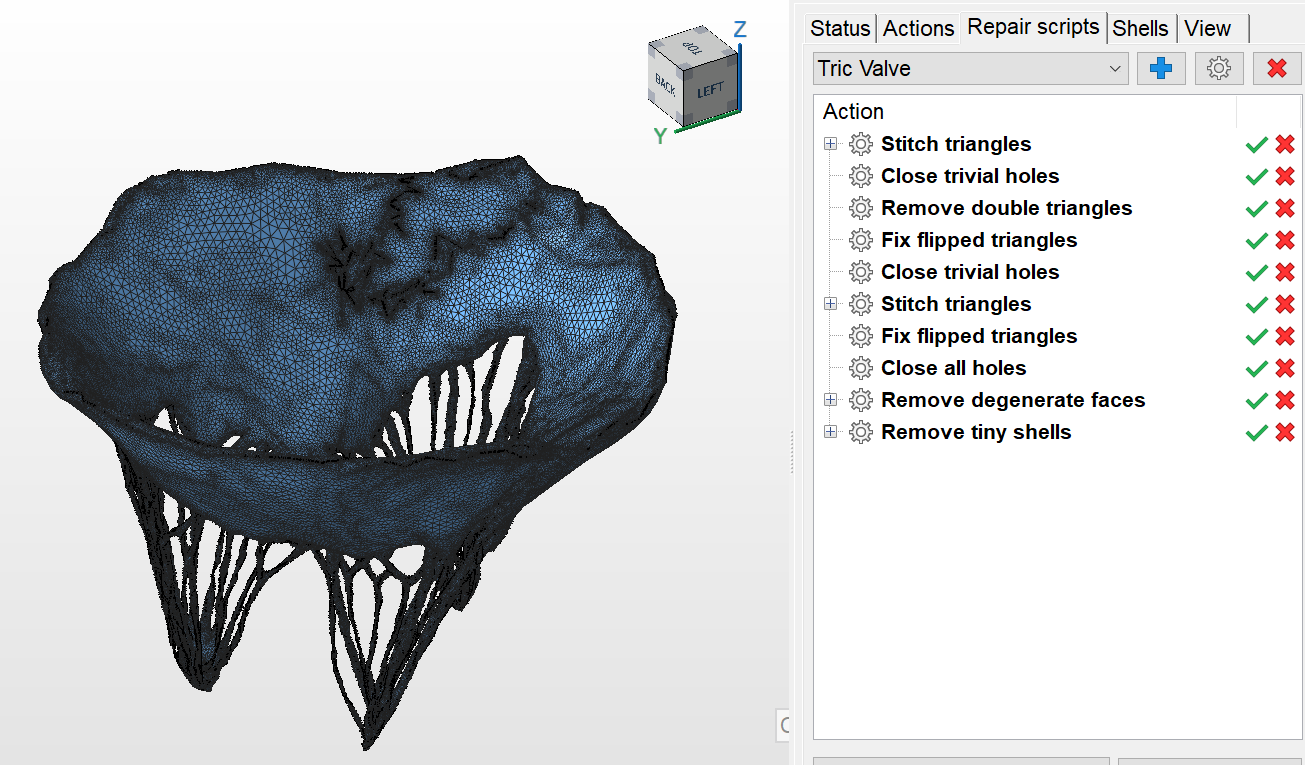
\includegraphics[width=0.8\textwidth]{figures/NetFabbRepair.png}
              \caption{Netfabb Repair Scripts}
              \label{fig:NetfabbRepair}
          \end{figure}
    \item Shell
          \begin{figure}
              \centering
              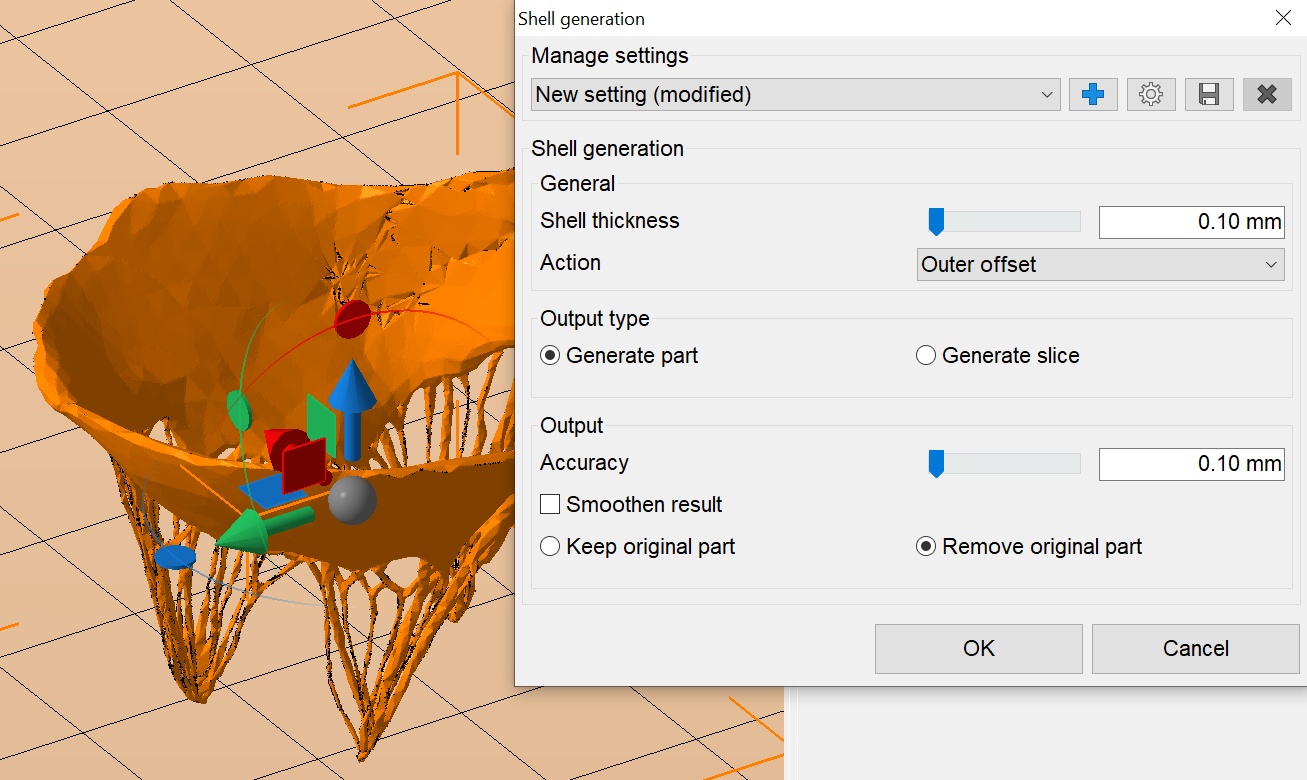
\includegraphics[width=0.8\textwidth]{figures/NetFabbShell.png}
              \caption{Netfabb Shell}
              \label{fig:NetfabbShell}
          \end{figure}
\end{itemize}


After the repairing and hollow shell process was completed the model was imported into Blender, here

Meshmixer was used in tandem with blender as it contained a very useful thickness analysis tool which could be used to see the varying thicknesses of the leaflets in the imported model, then Blender was used to manually edit the model using its sculpting tools to either thicken or thin the surface where appropriate.





Once the final valve model was finalised the decision was made to flatten the saddle-shape of the geometry to simplify the moulding and mounting processes, some surgical studies like \citeonly{mahmoodChangesMitralValve2010} showed that for mitral valves it does have a structural disadvantage however this did not reduce the ability to coapt properly.



% Physical prototyping:

% Printing errors
% Moulding errors
% Material errors
% Assembly errors
% Design errors


% Tools:

% 3D printer
% Spatula
% Syringe
% Precision blade
% Sanding paper
% Pliers
% Tweezers

\section{Prototyping}
\subsection{Valve Iterations}
\newthought{Preliminary Prototyping Methods}
The prototyping method went through a few key stages, throughout the simplified valve modelling stage the running methods were creating \gls{PLA} prints of the flat and balloon valve models and then using a silicone mould to capture its likeness, through feasability testing it was found this method was not suitable for reasons;
\begin{itemize}
    \item Silicone moulds could not hold firm enough in casting to maintain sub 1mm thicknesses
    \item The mould release agent was less effective on \gls{PU}-Silicone interfaces than expected
    \item The moulds even with appropriate ventilation would still have air bubbles and not fill out to the edges of the part.
\end{itemize}
As it seemed no amount of optimization of this method would improve results further work was done to find a more suitable method.

\newthought{Press Moulding}
This new method involved designing blocks in SolidWorks as a separate body to the valve part and using the 'Combine' tool to subtract the valve part. This hollowed block could then be split in the middle to create a two-part mould.

The \gls{PU} resin could then be poured into the cavity part and the lid part pressed ontop with a C-clamp to create a tight seal.

Some key considerations developed over trial and error for this method were:

\begin{itemize}
    \item Embossing and debossing key slots to ensure the moulds could be aligned correctly.
    \item Sanding down the \gls{PLA} prints to a smooth finish so in combination with a tailored mould release the casted part could be separated easily.
    \item Utilizing a vacuum chamber to remove air bubbles from the resin before curing.
\end{itemize}

% Materials used:

% Platinum cure silicone
% Polyurethane resin
% Ecolex transparent silicone
% Epoxy
% PLA
% SLA resin
% B7000 adhesive
% Nylon write
% Mould release
% Grease
% Isopropyl alcohol
\subsection{Chordae Tendineae }
Initial conceptualization of the chordae tendineae involved having the valve as one homogenous material with the tendineae attached within the mould. However, as the project progressed and the complexity of the valve increased, it was decided that the tendineae should be a separate part that could be attached after the valve was cast. This was decided on as the elastic modulus of the tendineae was vastly different as they function to be pulled taught to stop the leaflets from prolapsing.

\newthought{Design of Choice:}
A 0.1mm nylon fishing wire was chosen to represent the tendineae as it was thin enough to be completely collapsible and not interfere with the opening in the diastolic phase.

The attachment to the valve was the more challenging aspect, a few methods were considered and tested:
\begin{itemize}
    \item Suture patterns along the cusp of the leaflets.
          \begin{itemize}
              \item A short continuous suture was used to attach a few tendineae to the leaflets on a sample piece of \gls{PU} how on a gentle tensile test the suture ripped out as the \gls{PU} wasn't strong enough to hold.
          \end{itemize}
    \item Using a small hole in the leaflet to thread the tendineae through and then knotting it on the other side.
          \begin{itemize}
              \item This method also failed as the elasticity of the \gls{PU} made it so the knot would have to be \gls{PU} would rip anyway.
          \end{itemize}
    \item Embedding the wire in the \gls{PU} leaflets.
          \begin{itemize}
              \item While hopeful the embedding technique proved not feasible as the wire just slipped out, there was an attempt made with thick and thin layers of additional \gls{PU} but to no avail.
          \end{itemize}
    \item Gluing the tendineae to the leaflets with a cyanoacrylate adhesive.
          \begin{itemize}
              \item While this method showed initial promise as the adhesive was strong enough to hold the tendineae after seconds of curing, when 24 hours passed the adhesive would harden much stiffer and deform the leaflets making them very rigid.
          \end{itemize}
    \item Gluing with B7000 adhesive.
          \begin{itemize}
              \item The B7000 adhesive was chosen as it was a flexible adhesive, initial tests werent fruitful but if left to set fully over 24 hours the bond became very strong and the leaflets retained their flexibility while also only needing a miniscule amount for a good hold so the very thin thickness of the leaflets wasnt negated.
          \end{itemize}
\end{itemize}
\subsection{Fixturing}
The ideal design criterion was considered carefully before modelling the test fixturing. The main desired outcomes from the testing that the fixturing should facilitate were:

\begin{itemize}
    \item The chordae tendineae should have fixed anchors which are fully adjustable axially and angularly.
    \item The valve should be able to be mounted in a way that the leaflets are not obstructed and the valve can be viewed from all angles for through evaluation.
\end{itemize}

\newthought{Design of Choice:}
A combination of 3D printed parts, off-the-shelf components and hand-cut threaded rods were used to emulate the initial sketch of the rig

The threaded rods allowed for the anchoring points of the tendineae to be adjusted axially.

Attached to the rods was the ring system with notches that could be adjusted angularly which the mock tendineae were passed through and fastened to with a rubber wedge.